\documentclass[a4paper,10pt]{article}

\usepackage{tikz}
\usepackage{fullpage}
\usepackage{amsmath,amsthm,amsfonts,amssymb,amscd}
\usepackage{mathtools}
\usepackage{colortbl}
\usepackage{xcolor}
\usepackage{graphicx}
\usepackage{titlesec}
\usepackage{xepersian}
\usepackage{multirow}
\usepackage{caption}
\usepackage{fancyhdr}
\usepackage{mdframed}


% ---------------------------
%      Color Palette
% ---------------------------
\definecolor{BgDark}{HTML}{141420}
\definecolor{BgCard}{HTML}{1E1E2E}
\definecolor{AccentBlue}{HTML}{7AA2F7}
\definecolor{AccentPurple}{HTML}{BB9AF7}
\definecolor{AccentCyan}{HTML}{7DCFFF}
\definecolor{AccentGold}{HTML}{E0AF68}
\definecolor{TextPrimary}{HTML}{CDD6F4}
\definecolor{TextMuted}{HTML}{6C7086}
\definecolor{RuleLine}{HTML}{313244}

\pagecolor{BgDark}
\color{TextPrimary}


% ---------------------------
%  RTL-safe Info Box
% ---------------------------
\newmdenv[
backgroundcolor=BgCard,
fontcolor=TextPrimary,
linecolor=AccentBlue,
linewidth=1.2pt,
rightline=true,   % RTL: accent border on the RIGHT
leftline=false,
topline=false,
bottomline=false,
innerrightmargin=12pt,
innerleftmargin=12pt,
innertopmargin=10pt,
innerbottommargin=10pt,
skipabove=10pt,
skipbelow=10pt,
]{infobox}
% ---------------------------
%        Font Setup
% ---------------------------
\settextfont{Vazir.ttf}[
    BoldFont = Vazir-Bold.ttf,
    Path = fonts/
]
\setlatintextfont{Vazir.ttf}[
    BoldFont = Vazir-Bold.ttf,
    Path = fonts/
]

% ---------------------------
%     Custom Adjustments
% ---------------------------
\renewcommand{\baselinestretch}{1.2}
\renewcommand{\thesection}{\arabic{section}}

% User-defined commands for homework info (adjust as needed)
\newcommand{\HomeworkNumber}{1}
\newcommand{\HomeworkDeadline}{1405/01/14}
\newcommand{\id}{\texttt{\detokenize{@Amir_Hossein_Afshar}}}



\begin{document}

% ---------------------------------
%           Title Page
% ---------------------------------
\begin{titlepage}
	
	% Background decorations — right-side rectangle + gold horizontal line
	\begin{tikzpicture}[remember picture, overlay]
		% Right-side vertical rectangle (accent block)
		\fill[BgCard]
		([xshift=-2.2cm]current page.north east) rectangle
		(current page.south east);
		\draw[AccentGold!60, line width=0.8pt]
		([xshift=-2.2cm]current page.north east) --
		([xshift=-2.2cm]current page.south east);
	\end{tikzpicture}
	
	\vspace*{2.2cm}
	
	\begin{center}
		% Logo
		
\includegraphics[scale=1.05]{assets/fum-logo.png}\\[1.0cm]
		
		\textcolor{RuleLine}{\rule{8cm}{0.6pt}}\\[0.6cm]
		
		{\Huge \bfseries \textcolor{TextPrimary}{مبانی و کاربردهای هوش مصنوعی}}\\[0.4cm]
		
		\textcolor{RuleLine}{\rule{8cm}{0.6pt}}\\[0.4cm]
		
		{\large \textcolor{AccentCyan}{دانشگاه فردوسی مشهد}}\\[0.1cm]
		{\normalsize \textcolor{TextMuted}{گروه مهندسی کامپیوتر}}\\[0.2cm]
		{\normalsize \textcolor{AccentGold}{دکتر زارعی}}\\[1.6cm]
		{\normalsize \textcolor{TextMuted}{بهار 1405}}\\[0.2cm]
		
		% Homework number — simple, normal size
		{\normalsize \textcolor{TextMuted}{تمرین شماره}}
		{\large \bfseries \textcolor{AccentBlue}{\HomeworkNumber}}\\[1.4cm]
		
		% Deadline badge — gold border
		\setlength{\fboxrule}{0.8pt}%
		\fcolorbox{AccentGold!60}{BgCard}{%
			\begin{minipage}{7cm}
				\centering\vspace{5pt}
				\textcolor{AccentGold}{\bfseries مهلت تحویل: \HomeworkDeadline}
				\vspace{5pt}
			\end{minipage}
		}\\[0.8cm]
		
		% TA box — gold border
		\fcolorbox{AccentGold!60}{BgCard}{%
			\begin{minipage}{8cm}
				\centering\vspace{5pt}
				\textcolor{TextMuted}{مسئول تمرین:} \quad \textcolor{AccentCyan}{\id}
				\vspace{5pt}
			\end{minipage}
		}
	\end{center}
	
\end{titlepage}
% ---------------------------------
%          Instructions Page
% ---------------------------------
\clearpage

\vspace*{4pt}
\begin{center}
	\colorbox{BgCard}{%
		\begin{minipage}{\dimexpr\linewidth-2\fboxsep\relax}
			\centering
			\vspace{6pt}
			{\bfseries\large \textcolor{AccentGold}{دستورالعمل‌ها}}
			\vspace{6pt}
		\end{minipage}%
	}
\end{center}
\vspace{6pt}

\begin{infobox}
	دانشجویان محترم لطفا به موارد زیر توجه فرمایید:
	\begin{itemize}
		\itemsep0.4em
		\item
		تحویل تمرین‌ها فقط از طریق سامانه آموزش مجازی دانشگاه امکان‌پذیر است.
		\item
		تمرین‌ها باید دست‌نویس، خوانا و با استفاده از خودکار آبی یا مشکی و یا به صورت دیجیتالی با استفاده از قلم نوری نوشته شوند.
		\item
		از تمرین‌های حل‌شده دیگران استفاده نکنید. پیامدهای این کار با دانشجو می‌باشد.
		\item
		نوشتن جواب آخر به تنهایی نمره‌ای نداشته و تمام مراحل حل، مشمول نمره می‌باشد.
		\item
		به دلیل موعد از پیش تعیین‌شده تمرین‌ها و برنامه درسی، امکان تمدید تمرین وجود ندارد. همچنین ارسال تمرین پس از موعد تعیین‌شده نمره‌ای نخواهد داشت.
		\item
		نحوه نام‌گذاری فایل پاسخ باید مطابق جدول~\ref{tab:file_format} و به شکل \lr{\texttt{pdf}} باشد.
	\end{itemize}
	
	\vspace{10pt}
	
	% RTL-safe table: use center environment, manual column colors
	\begin{center}
		\arrayrulecolor{RuleLine}
		\begin{tabular}{|>{\columncolor{BgCard}\centering\arraybackslash}p{3cm}|>{\columncolor{BgDark}\centering\arraybackslash}p{7cm}|}
			\hline
			\textcolor{AccentCyan}{\bfseries\lr{Format}} &
			\texttt{\lr{StudentID-Full\_Name-\#HwNo.pdf}} \\
			\hline
			\textcolor{AccentGold}{\bfseries\lr{Example}} &
			\textcolor{TextMuted}{\texttt{\lr{9876543210-Alan\_Turing-\#01.pdf}}} \\
			\hline
		\end{tabular}
		\captionof{table}{\textcolor{TextMuted}{شیوه نام‌گذاری فایل‌ها}}
		\label{tab:file_format}
	\end{center}
	
\end{infobox}


\vspace{8pt}
\textcolor{AccentCyan}{\rule{\linewidth}{0.8pt}}
% ---------------------------------
%          questions
% ---------------------------------
%%%%%%%%%%%%%%%%%%%%%%%%%%%%%%%%%%%%%%%%%%%%%%%%%%%%%%%%%%%%%%%%%%%%%%%%%%%%%%%%%%%%%%%%%%%%%%
\section{\textcolor{AccentGold}{سوال اول}}
درستی و نادرستی موارد زیر را مشخص کنید و دلیل آن را بیان کنید.
\begin{itemize}
	\item 
	الف) عامل واکنشی ساده (
	\lr{simple reflective agent}
	)
	در محیط های 
	\lr{partially observable}
	کارایی ندارد.
	\item 
	ب)
	عامل واکنشی ساده (
	\lr{simple reflective agent}
	)
	در محیط های پویا کارایی ندارد.
	\item 
	پ)
	از میان انواع عامل ها، فقط عامل های واکنشی ساده وضعیت دنیا را ذخیره نمی کنند.
	\item 
	ت) 
	عاملی که تخته نرد بازی می کند در محیطی ایستا، قطعی، مشاهده پذیر، گسسته و واقعه ای می باشد.
	
\end{itemize}
\bigskip
\textcolor{AccentCyan}{\rule{\linewidth}{0.4pt}}
%%%%%%%%%%%%%%%%%%%%%%%%%%%%%%%%%%%%%%%%%%%%%%%%%%%%%%%%%%%%%%%%%%%%%%%%%%%%%%%%%%%%%%%%%%%%%%
\section{\textcolor{AccentGold}{سوال دوم}}
در رابطه با انواع عامل ها، به موارد زیر پاسخ دهید.
\begin{itemize}
	\item 
	الف) اگر هدف رساندن یک مسافر به مقصد توسط یک عامل هوشمند باشد و معیار کارایی، امینت، زمان و مسیر خلوت باشد، چه نوع عاملی مناسب است؟
	\item 
	ب) روبات برف پاک کن هوشمندی در خودرو در اختیار داریم. این ربات، در کدام دسته از عامل های هوشمند قرار می گیرد؟
\end{itemize}

\bigskip
\textcolor{AccentCyan}{\rule{\linewidth}{0.4pt}}
%%%%%%%%%%%%%%%%%%%%%%%%%%%%%%%%%%%%%%%%%%%%%%%%%%%%%%%%%%%%%%%%%%%%%%%%%%%%%%%%%%%%%%%%%%%%%%
\section{\textcolor{AccentGold}{سوال سوم}}
گراف زیر را در نظر بگیرید. گره A وضعیت شروع و گره F وضعیت هدف را نشان می دهند. با استفاده از روش جست و جوی UCS درخت جست و جو را رسم کنید و همچنین ترتیب ملاقات گره ها را بیان کنید.

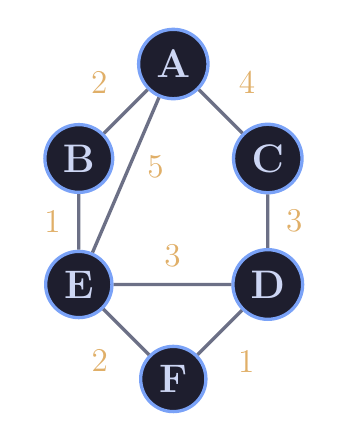
\begin{tikzpicture}[
	scale=0.8, % Overall scale of the graph
	% Style for the circular nodes
	main node/.style={
		circle,
		draw=AccentBlue,      % Node border color
		fill=BgCard,          % Node background color
		text=TextPrimary,     % Node text color
		very thick,
		minimum size=8mm,
		font=\Large\bfseries
	},
	% Style for the lines connecting the nodes
	edge/.style={
		draw=TextMuted,       % Using TextMuted so it's visible on BgDark
		very thick
	},
	% Style for the numbers on the edges
	weight/.style={
		text=AccentGold,      % Golden color for weights to stand out
		font=\large\bfseries,
		inner sep=6pt         % Spacing between text and the line
	}
	]
	
	% 1. Define Node Positions (Coordinates form a nice symmetric shape)
	\node[main node] (A) at (0, 2) {A};
	\node[main node] (B) at (-1.5, 0.5) {B};
	\node[main node] (C) at (1.5, 0.5) {C};
	\node[main node] (E) at (-1.5, -1.5) {E};
	\node[main node] (D) at (1.5, -1.5) {D};
	\node[main node] (F) at (0, -3) {F};
	
	% 2. Draw Edges and Place Weight Labels
	\draw[edge] (A) -- node[weight, above left] {$2$} (B);
	\draw[edge] (A) -- node[weight, above right] {$4$} (C);
	\draw[edge] (A) -- node[weight, right, pos=0.45] {$5$} (E);
	
	\draw[edge] (B) -- node[weight, left] {$1$} (E);
	
	\draw[edge] (C) -- node[weight, right] {$3$} (D);
	
	\draw[edge] (E) -- node[weight, above] {$3$} (D);
	\draw[edge] (E) -- node[weight, below left] {$2$} (F);
	
	\draw[edge] (D) -- node[weight, below right] {$1$} (F);
	
\end{tikzpicture}

\bigskip
\textcolor{AccentCyan}{\rule{\linewidth}{0.4pt}}
%%%%%%%%%%%%%%%%%%%%%%%%%%%%%%%%%%%%%%%%%%%%%%%%%%%%%%%%%%%%%%%%%%%%%%%%%%%%%%%%%%%%%%%%%%%%%%
\section{\textcolor{AccentGold}{سوال چهارم}}
در مسئله زیر، برای رسیدن از S به G با استفاده از روش جست و جوی UCS و با استفاده از حالت جست و جوی گرافی، درخت جست و جو را رسم کنید و ترتیب پیمایش گره ها را بیان کنید.

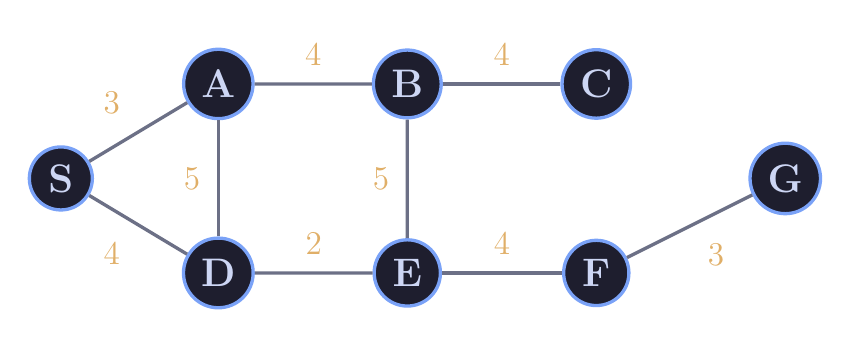
\begin{tikzpicture}[
	scale=0.8, % Adjusted scale for the wider horizontal layout
	% Style for the circular nodes
	main node/.style={
		circle,
		draw=AccentBlue,      
		fill=BgCard,          
		text=TextPrimary,     
		very thick,
		minimum size=8mm,
		font=\Large\bfseries
	},
	% Style for the lines connecting the nodes
	edge/.style={
		draw=TextMuted,       
		very thick
	},
	% Style for the numbers on the edges
	weight/.style={
		text=AccentGold,      
		font=\large\bfseries,
		inner sep=6pt         
	}
	]
	
	% 1. Define Node Positions (Horizontal layout matching the image)
	\node[main node] (S) at (0, 0) {S};
	
	\node[main node] (A) at (2.5, 1.5) {A};
	\node[main node] (D) at (2.5, -1.5) {D};
	
	\node[main node] (B) at (5.5, 1.5) {B};
	\node[main node] (E) at (5.5, -1.5) {E};
	
	\node[main node] (C) at (8.5, 1.5) {C};
	\node[main node] (F) at (8.5, -1.5) {F};
	
	\node[main node] (G) at (11.5, 0) {G};
	
	% 2. Draw Edges and Place Weight Labels
	% From Start node S
	\draw[edge] (S) -- node[weight, above left] {$3$} (A);
	\draw[edge] (S) -- node[weight, below left] {$4$} (D);
	
	% Vertical edges
	\draw[edge] (A) -- node[weight, left] {$5$} (D);
	\draw[edge] (B) -- node[weight, left] {$5$} (E);
	
	% Top horizontal edges
	\draw[edge] (A) -- node[weight, above] {$4$} (B);
	\draw[edge] (B) -- node[weight, above] {$4$} (C);
	
	% Bottom horizontal edges
	\draw[edge] (D) -- node[weight, above] {$2$} (E);
	\draw[edge] (E) -- node[weight, above] {$4$} (F);
	
	% To Goal node G
	\draw[edge] (F) -- node[weight, below right] {$3$} (G);
	
\end{tikzpicture}

\bigskip
\bigskip
\textcolor{AccentCyan}{\rule{\linewidth}{0.4pt}}
%%%%%%%%%%%%%%%%%%%%%%%%%%%%%%%%%%%%%%%%%%%%%%%%%%%%%%%%%%%%%%%%%%%%%%%%%%%%%%%%%%%%%%%%%%%%%%
\section{\textcolor{AccentGold}{سوال پنجم}}

فرض کنید در یک مسئله جست و جو، فضای جست و جو یک درخت محدود باشد که در آن هزینه هر یال یک عدد گویا است (هزینه ها می توانند منفی باشند.) در این صورت، از میان همه روش های جست و جوی ناآگاهانه، کدام روش می تواند مسیر بهینه را پیدا کند؟

\bigskip
\textcolor{AccentCyan}{\rule{\linewidth}{0.4pt}}
%%%%%%%%%%%%%%%%%%%%%%%%%%%%%%%%%%%%%%%%%%%%%%%%%%%%%%%%%%%%%%%%%%%%%%%%%%%%%%%%%%%%%%%%%%%%%%
\section{\textcolor{AccentGold}{سوال ششم}}
در حین انجام یک روش جست و جو، درخت  جست و جوی حاصل به شکل مقابل رشد یافته است. راس هایی که نامزد بسط داده شدن هستند با رنگ آبی نمایش داده شده اند. بررسی کنید کدام یک از جست و جوهای زیر، می تواند روش جست و جو باشد.

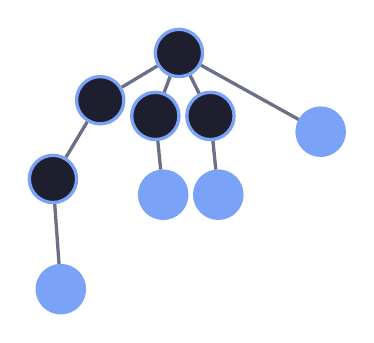
\begin{tikzpicture}[
	scale=1, % Scale of the tree
	% Style for the empty/hollow nodes
	empty node/.style={
		circle,
		draw=AccentBlue,      % Border color
		fill=BgCard,          % Inner color matching the dark theme
		very thick,
		minimum size=6mm,     % Slightly smaller since there's no text
		inner sep=0pt
	},
	% Style for the filled/solid nodes
	solid node/.style={
		circle,
		draw=AccentBlue,      % Border color
		fill=AccentBlue,      % Completely filled with accent color
		very thick,
		minimum size=6mm,
		inner sep=0pt
	},
	% Style for the connecting lines
	edge/.style={
		draw=TextMuted,
		very thick
	}
	]
	
	% 1. Define Node Positions (Root and Levels)
	% Root
	\node[empty node] (root) at (0, 0) {};
	
	% Level 1 (Left to Right)
	\node[empty node] (l1_1) at (-1.0, -0.6) {};
	\node[empty node] (l1_2) at (-0.3, -0.8) {};
	\node[empty node] (l1_3) at (0.4, -0.8) {};
	\node[solid node] (l1_4) at (1.8, -1.0) {};
	
	% Level 2
	\node[empty node] (l2_1) at (-1.6, -1.6) {}; % Child of leftmost node
	\node[solid node] (l2_2) at (-0.2, -1.8) {}; % Child of second node
	\node[solid node] (l2_3) at (0.5, -1.8) {};  % Child of third node
	
	% Level 3
	\node[solid node] (l3_1) at (-1.5, -3.0) {}; % Child of the far-left branch
	
	% 2. Draw Edges connecting the nodes
	% Edges from root
	\draw[edge] (root) -- (l1_1);
	\draw[edge] (root) -- (l1_2);
	\draw[edge] (root) -- (l1_3);
	\draw[edge] (root) -- (l1_4);
	
	% Edges from Level 1 to Level 2
	\draw[edge] (l1_1) -- (l2_1);
	\draw[edge] (l1_2) -- (l2_2);
	\draw[edge] (l1_3) -- (l2_3);
	
	% Edge from Level 2 to Level 3
	\draw[edge] (l2_1) -- (l3_1);
	
\end{tikzpicture}
\begin{itemize}
	\item 
	DFS
	\item 
	BFS
	\item 
	UCS
	\item 
	\lr{
	Iterative Deepening Search}
\end{itemize}
\bigskip
\textcolor{AccentCyan}{\rule{\linewidth}{0.4pt}}
%%%%%%%%%%%%%%%%%%%%%%%%%%%%%%%%%%%%%%%%%%%%%%%%%%%%%%%%%%%%%%%%%%%%%%%%%%%%%%%%%%%%%%%%%%%%%%


% Add more sections as needed...

\end{document}
